\documentclass{beamer}

\mode<presentation> {
	\usetheme{Madrid}
}

\usepackage{graphicx} % Allows including images
\usepackage{booktabs} % Allows the use of \toprule, \midrule and \bottomrule in tables

%----------------------------------------------------------------------------------------
%	TITLE PAGE
%----------------------------------------------------------------------------------------

\title[Data mining religiosity measurements]{Synthesizing a better religiosity measure} % The short title appears at the bottom of every slide, the full title is only on the title page

\author{William Guo} % Your name
\institute{ Rice University }
\date{\today} % Date, can be changed to a custom date

\begin{document}

\begin{frame}
	\titlepage % Print the title page as the first slide
\end{frame}

%----------------------------------------------------------------------------------------
%	PRESENTATION SLIDES
%----------------------------------------------------------------------------------------

\begin{frame}
\frametitle{Initial concerns}
\begin{itemize}
	\item Traditional measures of religiosity suffer from misclassifying the growing secular population around the world
	\item Many of the questions about religion are more biased towards a Western audience, e.g. church attendance, belief in Hell
	\item \textbf{Question:} how can we disentangle religious denomination from measures of religiosity? 
\end{itemize}
\end{frame}

%----------------------------------------------------------------------------------------

\begin{frame}
\frametitle{Motivation}
\begin{itemize}
	\item When measuring religiosity, there is a tradeoff between how easy a question is to measure and how accurately it pinpoints one's true religiosity
	\begin{itemize}
		\item E.g. attendance is easily measured, but is not comparable between members of different religions
		\item On the other hand, more ambiguous questions that can address many different religions are then less quantifiable
	\end{itemize}
	\item Adding more variables will decrease the interpretability of our models
\end{itemize}
\end{frame}

%----------------------------------------------------------------------------------------

\begin{frame}
	\frametitle{Solution}
	\begin{itemize}
		\item \large We can synthesize our own variables through factor analysis!
	\end{itemize}
\end{frame}

%----------------------------------------------------------------------------------------

\begin{frame}
	\frametitle{Exploratory data analysis}
	\begin{itemize}
		\item Performed t-SNE on a group of questions in the WVS regarding religion and ethics to visualize whether any denomination-based clusters emerged from the data
		\begin{itemize}
			\item Finds and minimizes the KL-divergence between the joint probability distribution of two points in the original, high-dimension space and two points in the lower-dimensional space (usually 2D for visualization purposes)
		\end{itemize}
		\item \textbf{Question:} do we expect members of one religion to answer differently from another's?
	\end{itemize}
\end{frame}

%----------------------------------------------------------------------------------------

\begin{frame}
	\frametitle{Exploratory data analysis (cont.)}
	\begin{center}
		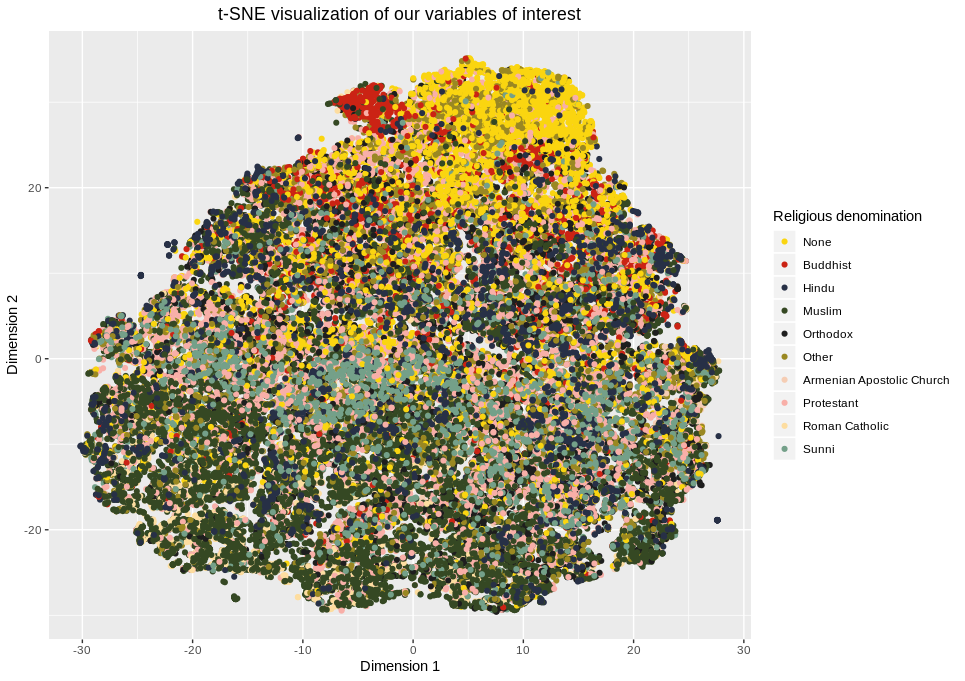
\includegraphics[width=0.9\textwidth]{tsne.png}
	\end{center}
\end{frame}

%----------------------------------------------------------------------------------------

\begin{frame}
\frametitle{Dimensionality reduction}
	\begin{itemize}
		\item PCA is not quite theoretically sound due to the fact that we are dealing with categorical variables and it requires scaled data
		\item Instead, I use multiple correspondence analysis (MCA)
		\begin{itemize}
			\item Performs singular value decomposition on the indicator matrix of the data (instead of the covariance matrix like in PCA)
			\item In essence, makes dummy variables out of the original variables
			\item Could have achieved a similar result by binarizing the data by hand and running PCA on it
		\end{itemize}
	\end{itemize}
\end{frame}

%----------------------------------------------------------------------------------------

\begin{frame}
	\frametitle{Dimensionality reduction (cont.)}
	\begin{columns}
		\begin{column}{0.55\textwidth}
			\begin{center}
				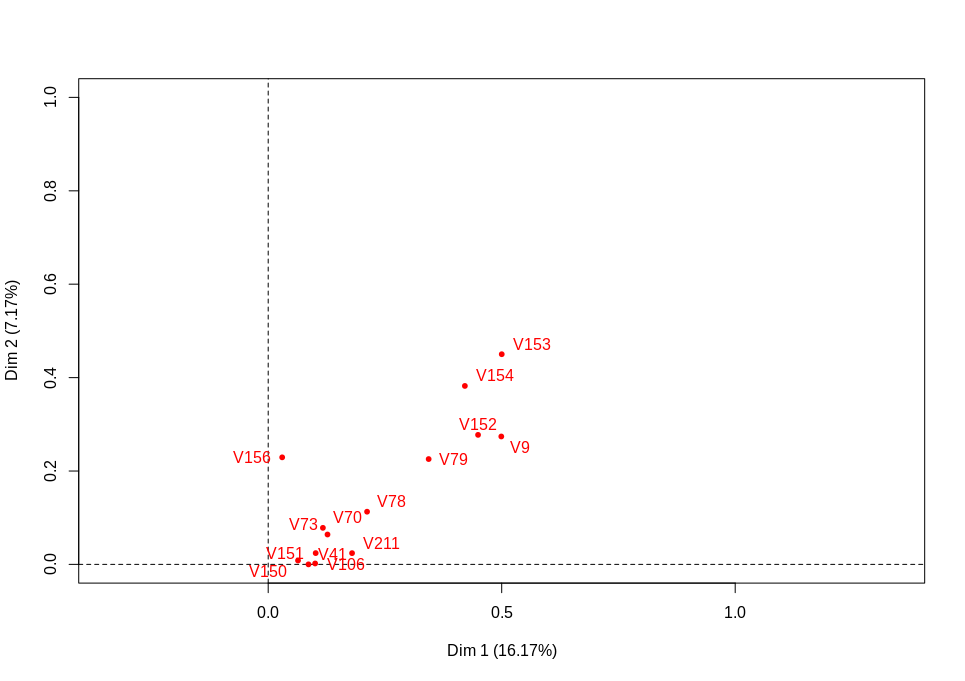
\includegraphics[width=\textwidth]{mca_corr.png}
			\end{center}
		\end{column}
		\begin{column}{0.45\textwidth}  %%<--- here
			\begin{center}
				\begin{center}
					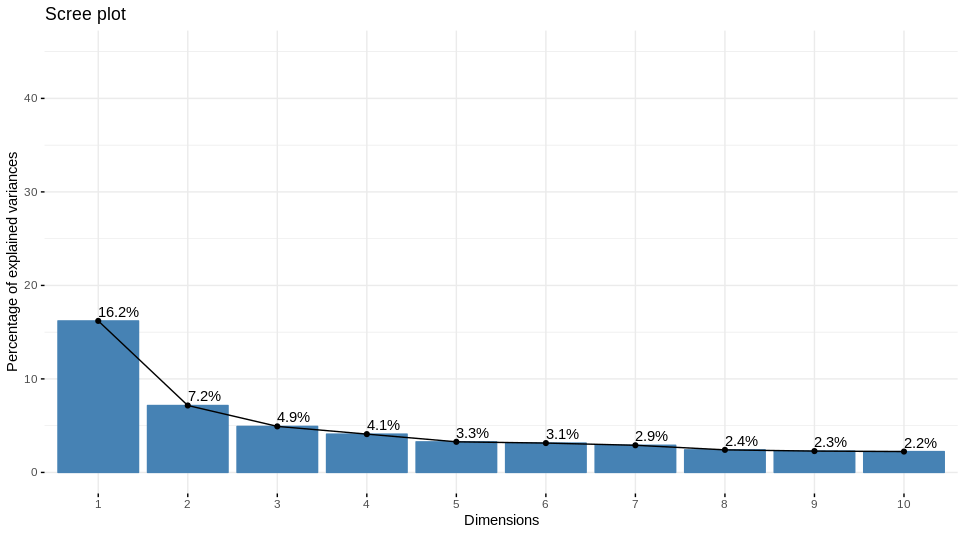
\includegraphics[width=\textwidth]{mca_scree.png}
				\end{center}
			\end{center}
		\end{column}
	\end{columns}
\end{frame}

%------------------------------------------------

\begin{frame}
	\frametitle{Model proposition}
	\begin{itemize}
		\item First dimension explains the person's religious feelings (\texttt{inner}) 
		\begin{itemize}
			\item V150 and V151 ask the subject their opinion on the purpose of religion (existential, uphold traditions, do good things)
			\item V73 asks if it is important to spoil oneself
			\item V211 asks if they are proud of their nationality 
		\end{itemize}
		\item Second dimension deals more with how the person feels about people of different religions (\texttt{outer})
		\begin{itemize}
			\item V156 asks the subject if people of other religions are just as moral as their religion's members
			\item V153 deals with whether religion is superior to science when they conflict
			\item V154 questions whether the only acceptable religion is one's own
		\end{itemize}
	\end{itemize}
\end{frame}

%------------------------------------------------

\begin{frame}
	\frametitle{Regression results}
	\begin{table}[!htbp] \centering 
		\tiny
		\resizebox{0.6\linewidth}{!}{ 
			\begin{tabular}{@{\extracolsep{5pt}}lcc} 
				\\[-1.8ex]\hline 
				\hline \\[-1.8ex] 
				& \multicolumn{2}{c}{\textit{Dependent variable:}} \\ 
				\cline{2-3} 
				\\[-1.8ex] & \texttt{inner} & \texttt{outer} \\ 
				\\[-1.8ex] & \textit{OLS} & \textit{instrumental} \\ 
				& \textit{} & \textit{variable} \\ 
				\\[-1.8ex] & (1) & (2)\\ 
				\hline \\[-1.8ex] 
				age & 0.004$^{***}$ &  \\ 
				& (0.0001) &  \\ 
				& & \\ 
				sex & 0.007$^{*}$ &  \\ 
				& (0.004) &  \\ 
				& & \\ 
				educ & 0.048$^{***}$ &  \\ 
				& (0.001) &  \\ 
				& & \\ 
				inc\_ineq &  & $-$0.029$^{***}$ \\ 
				&  & (0.007) \\ 
				& & \\ 
				gov\_resp &  & 0.006$^{***}$ \\ 
				&  & (0.002) \\ 
				& & \\ 
				unreg\_comp &  & $-$0.008$^{***}$ \\ 
				&  & (0.001) \\ 
				& & \\ 
				Constant & $-$0.448$^{***}$ & 0.161$^{***}$ \\ 
				& (0.010) & (0.033) \\ 
				& & \\ 
				\hline \\[-1.8ex] 
				Observations & 55,140 & 55,140 \\ 
				R$^{2}$ & 0.063 & $-$0.027 \\ 
				Adjusted R$^{2}$ & 0.063 & $-$0.027 \\ 
				Residual Std. Error (df = 55136) & 0.465 & 0.397 \\ 
				F Statistic & 1,243.375$^{***}$ (df = 3; 55136) &  \\ 
				\hline 
				\hline \\[-1.8ex] 
				\textit{Note:}  & \multicolumn{2}{r}{$^{*}$p$<$0.1; $^{**}$p$<$0.05; $^{***}$p$<$0.01} \\ 
			\end{tabular} 
		}
	\end{table} 
\end{frame}

%------------------------------------------------
\begin{frame}
	\frametitle{Big takeaways}
	\begin{itemize}
		\item Data exploration showed some small clusters, but on the whole shows that religious denomination was a poor way to cluster the responses 
		\item MCA was unable to sufficiently explain the variance in the subjects' responses
		\item Coefficients are all very significant, but are also very small and do not explain the highest-variance components of the religious questions
	\end{itemize}
\end{frame}

%------------------------------------------------
\begin{frame}
\frametitle{Future work}
	\begin{itemize}
		\item Find a better algorithm that can create better components
		\item Work with different variables
	\end{itemize}
\end{frame}

%------------------------------------------------

\end{document} 